\documentclass[justified]{article}

\usepackage{amsmath, amsfonts, amssymb, amsthm}
\usepackage{enumerate}
\usepackage[margin=1.1in]{geometry}
\usepackage{graphicx}
\usepackage{hyperref}

\usepackage{float}
\usepackage{microtype}
\usepackage{mathpazo}
\usepackage{tikz}

\hypersetup{
    colorlinks=true,
    linkcolor=blue,
    citecolor=blue,
    urlcolor=blue,
}

\urlstyle{same}

\tikzstyle{circleblock} = [draw, fill=white, circle, inner sep=0]

\begin{document}
  \title{Data Preprocessing for Noise-Resistant CNNs}
  \author{Rowen Hunter, Eero Gallano, Jonathan Lee}
  \date{\today}
  \maketitle

  \section{Problem Statement and Background}
  % Motivation, related work, summary of contribution, results

  The problem we tackled was computer vision classification, where real world images are identified with a neural network.
  The largest hurdle in this project was we don’t know what images the network will be tested on; they may be perturbed, warped and noisy. So, the main priority for this project was building a classifier that is robust enough to handle any of those disturbances, and produce accurate results regardless. Robust image classification is an important problem in many fields, such as self driving cars, where signs need to be identified just as accurately on a rainy or foggy day as on a bright sunny one, and in automated moderation, where unsuitable imagery needs to be detected and removed even if its been overlaid or filtered.

  We considered a number of computer vision models and architectures to approach this problem, including Mobilenet \cite{Sandler_2018}, Resnet \cite{7780459}, Alexnet \cite{NIPS2012_4824}, VGG \cite{simonyan2014deep}, and DenseNet \cite{i2014densenet}. All of these models have been trained on, and performed well on, the ImageNet dataset. Our project dataset, Tiny ImageNet, is a sort of scaled down version of that dataset, so we thought it would be a good jumping off point.

  \subsection{Datasets and Metrics}

  The dataset we used is the tiny ImageNet dataset, which is already partitioned into training, test, and validation sets containing 100,000, 10,000, and 10,000 samples each, respectively.
  Each sample is a $64 \times 64$ RGB image that can belong to one of 200 classes.
  Nearly all the images are natural (photographs) and not synthetic, so most images have spectral content concentrated around low frequencies.

  \begin{figure}[H]
    \centering
    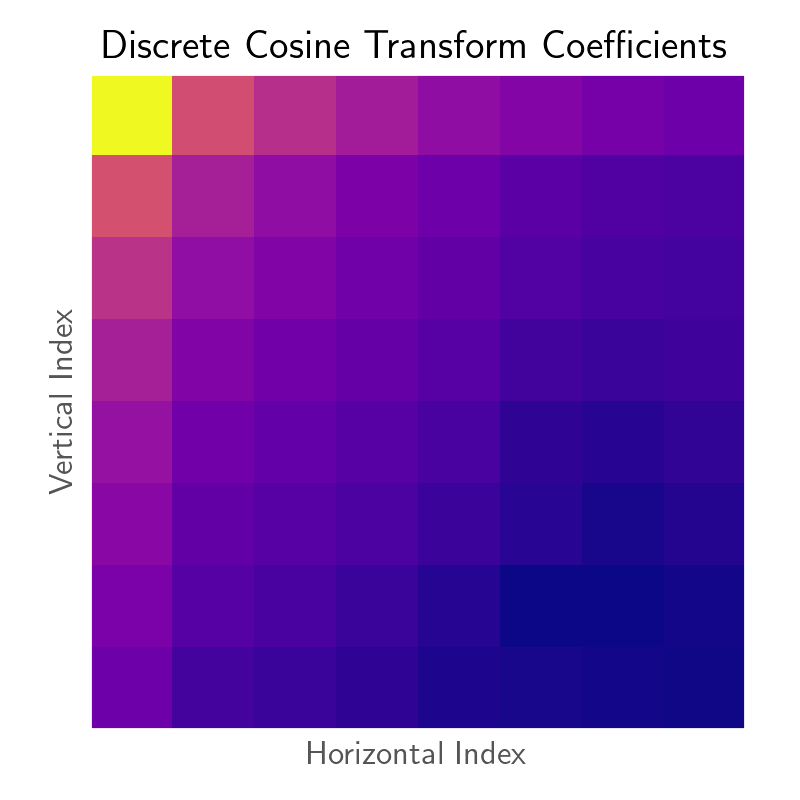
\includegraphics[width=0.5\textwidth]{figures/dct}
    \caption{
      Average power spectrum (on a $\log_{10}$-scale) of $8 \times 8$ blocks from 200 randomly selected images from the training set.
      Obtained by mapping each image into a luminescence layer and taking the Discrete Cosine Transform (DCT) of each block.
      The upper left corner depicts strong DC content in both spatial dimensions, and the lower right corner depicts sparse high-frequency content.
    }
  \end{figure}

  The metrics we considered for the classifier were top-1 and top-5 accuracy on the validation set.
  For the auxiliary denoising network that we will describe, we considered the peak signal-to-noise ratio (PSNR)---a proxy for mean squared error (MSE)---between a reference image and output image.

  \section{Approach}
  % Assumptions, definitions, objective

  \subsection{Data Augmentation}

  In natural images, rotations, translations, and variations in color occur regularly due to camera positioning and lighting conditions.
  To encourage our classifier to be invariant to these perturbations, we augmented the training dataset by randomly perturbing each sample image with probability 0.5. If perturbed, the image was subjected to the following transformations:
  \begin{enumerate}
  \item
    \textbf{Spatial perturbations} consisted of horizontal and vertical reflections, each occurring independently with probability $0.5$, and either a rotation or a crop, which were equally likely:
    \begin{enumerate}[(i)]
    \item
      A rotation involved padding the image by 60 pixels on all sides using reflection, rotating by a random number of degrees (uniformly chosen in the range $-180^\circ, +180^\circ$), and cropping to the centermost $224 \times 224$ pixels.
      The padding ensures the corners of the rotated image are always filled with pixels that resemble the boundary of the original image, as opposed to having those unused pixels zeroed out.

    \item
      A crop selects a region, between half and unit scale, with an aspect ratio between $\frac{3}{4}$ and $\frac{4}{3}$ of that of the original image.
      This region is then resize to fit the original image, which can introduce distortion along each spatial axis.
    \end{enumerate}

  \item
    \textbf{Color perturbations} consisted of modifying the brightness, contrast, saturation, and hue by $\pm 50\%$, $\pm 30\%$, $\pm 30\%$, and hue factor $\pm 0.05$, respectively, and adding zero-mean Gaussian noise to each channel of every pixel.
    Each channel value ranges between 0 and 1, so we chose 0.1 as the noise standard deviation.
    These variations were chosen heuristically so that the perturbed images sufficiently resembled the source image.
    The purpose of the Gaussian noise is to model high-frequency content that characterizes misclassified inputs in gradient-based attacks.
  \end{enumerate}

  \begin{figure}[H]
    \centering
    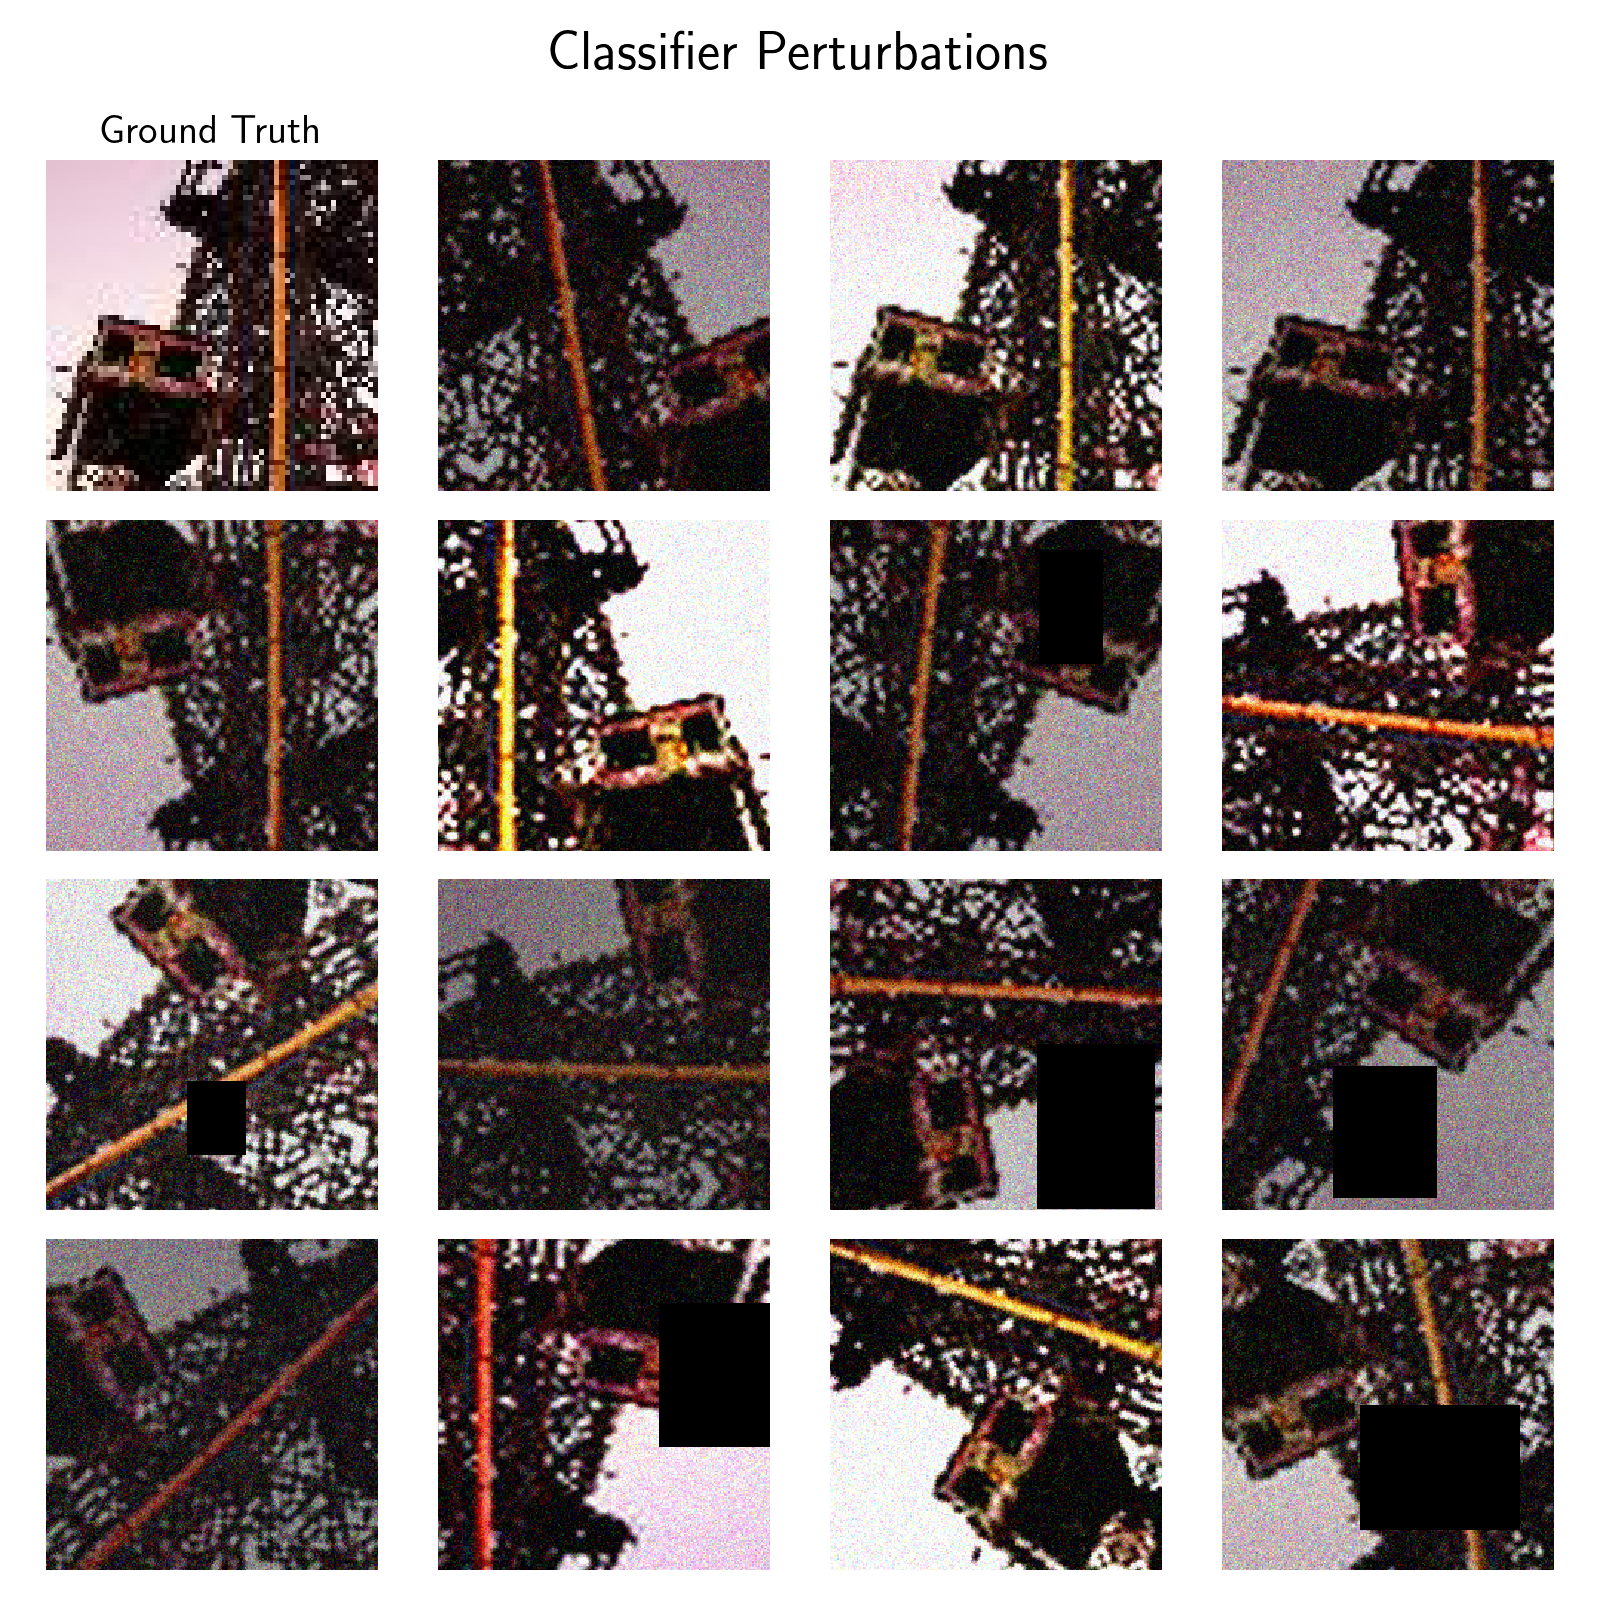
\includegraphics[width=0.8\textwidth]{figures/perturb.png}
    \caption{
      Example of randomly applied spatial and color perturbations.
      The original image (ground truth) is shown in the upper left corner.
    }
  \end{figure}

  We also tried random erasures, where randomly selected boxes of pixels were colored black.
  Like dropout, the erasures would encourage the classifier to learn a diverse set of features, leading to better generalization.
  However, in practice, the erasures often hid portions of the image salient to classification and the classifier was effectively training on very noisy images.
  We can view erasure as a very strong regularizer that hindered the ability of the network effectively, causing validation accuracy to plateau.

  \subsection{Models}

  \subsubsection{Classifier}

  Existing deep neural networks for image classification already offer very good feature extraction for generic tasks.
  Therefore, we used

  \subsubsection{Denoising Network}

  In signal processing, it is common to use filters, often designed by hand using domain knowledge to meet some specifications, to reduce noise in the raw data and make analyses more interpretable.
  Inspired by this paradigm, we introduced a small CNN with residual connections---a denoising network---to preprocess images before classification.

  The denoising network architecture shown in Figure \ref{fig:denoise}) attempts to undo the color perturbations introduced during data augmentation.
  The network's loss function is the MSE between $I_0$, a reference image without the color perturbation $\delta I$, and the network output $I$.
  We can use the MSE to estimate the PSNR, a nonnegative quantity measured in decibels (dB) that increases as $I \to I_0$ (\textit{i.e.}, the denoising network undoes the perturbation $\delta I$) and goes to zero when the MSE is maximized.
  \begin{equation}
    \begin{split}
      \mathsf{MSE}(I_0, I) &= \frac{1}{224 \times 224} \sum_{(x, y, c)} \left(I_0(x, y, c) - I(x, y, c)\right)^2 \leq 3^2 \\
      \mathsf{PSNR}(I_0, I) &= 10 \log_{10} \left(\frac{3^2}{\mathsf{MSE}(I_0, I)}\right)
    \end{split}
  \end{equation}
  $I_0(x, y, c) \in [0, 1]$ denotes the reference image's value at row $1 \leq y \leq 224$, column $1 \leq x \leq 224$, and channel $1 \leq c \leq 3$.

  \begin{figure}[H]
    \centering
    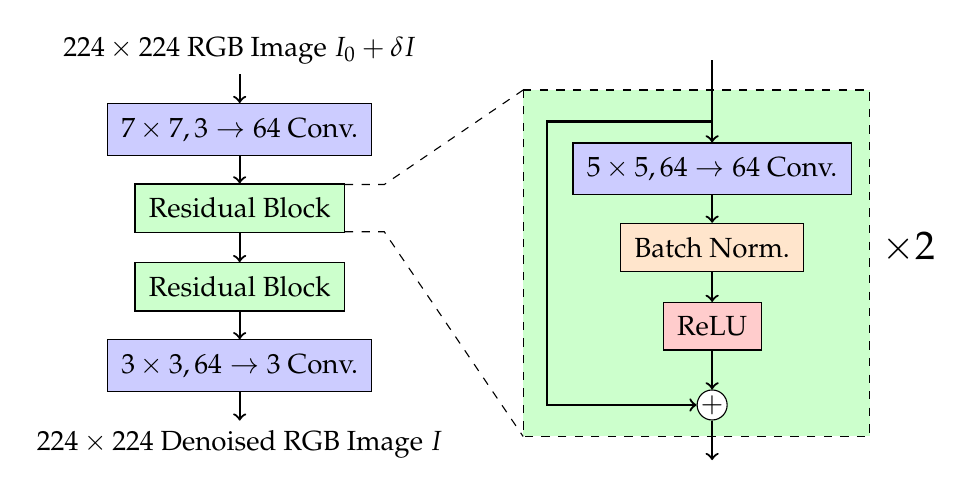
\begin{tikzpicture}
      \node (input) at (0, 0) {$224 \times 224$ RGB Image $I_0 + \delta I$};
      \node[draw, fill=blue!20, inner sep=5pt] (conv7x7) at (0, -1) {$7 \times 7, 3 \to 64$ Conv.};
      \node[draw, fill=green!20, inner sep=5pt] (resid1) at (0, -2) {Residual Block};
      \node[draw, fill=green!20, inner sep=5pt] (resid2) at (0, -3) {Residual Block};
      \node[draw, fill=blue!20, inner sep=5pt] (conv3x3) at (0, -4) {$3 \times 3, 64 \to 3$ Conv.};
      \node (output) at (0, -5) {$224 \times 224$ Denoised RGB Image $I$};
      \fill[green!20] (3.6, -0.5) rectangle (8, -4.9);

      \node (blockin) at (6, 0) {};
      \node[draw, fill=blue!20, inner sep=5pt] (conv5x5) at (6, -1.5) {$5 \times 5, 64 \to 64$ Conv.};
      \node[draw, fill=orange!20, inner sep=5pt] (batchnorm) at (6, -2.5) {Batch Norm.};
      \node[draw, fill=red!20, inner sep=5pt] (relu) at (6, -3.5) {ReLU};
      \node (blockout) at (6, -5) {};
      \node at (8.5, -2.5) {\Large $\times 2$};
      \node[circleblock] (sum) at (6, -4.5) {$+$};

      \draw[->, thick] (input) -- (conv7x7);
      \draw[->, thick] (conv7x7) -- (resid1);
      \draw[->, thick] (resid1) -- (resid2);
      \draw[->, thick] (resid2) -- (conv3x3);
      \draw[->, thick] (conv3x3) -- (output);

      \draw[->, thick] (blockin) -- (conv5x5);
      \draw[->, thick] (conv5x5) -- (batchnorm);
      \draw[->, thick] (batchnorm) -- (relu);
      \draw[->, thick] (relu) -- (sum);
      \draw[->, thick] (sum) -- (6, -5.2);
      \draw[dashed] (3.6, -0.5) -- (8, -0.5) -- (8, -4.9) -- (3.6, -4.9) -- (3.6, -0.5);
      \draw[dashed] (resid1.east) ++ (0, 0.3) -- ++(0.5, 0) -- (3.6, -0.5);
      \draw[dashed] (resid1.east) ++ (0, -0.3) -- ++(0.5, 0) -- (3.6, -4.9);
      \draw[->, thick] (6, -0.9) -- (3.9, -0.9) -- (3.9, -4.5) -- (sum);
    \end{tikzpicture}
    \caption{
      Denoising network architecture.
      All convolutional blocks use stride 1 and padding such that the spatial dimensions are preserved.
    }
    \label{fig:denoise}
  \end{figure}

  %+ Additive white Gaussian noise layers?
  % denoising layers?
  % compression?
  % ensembles
  % \item FGSM-generated samples

  \section{Results}

  \subsection{Denoising Network}

  We trained the denoising network with the Adam optimizer, with a learning rate of $10^{-5}$, exponential learning rate decay of $0.9$ per epoch, weight decay of $10^{-5}$, and batch size of $16$.
  Given that the model is relatively simple and that the loss plateaus, we only needed to train the network for two epochs.
  The training PSNR over time is shown in Figure \eqref{fig:denoise-psnr} (the $\log_{10}$ scale better captures changes in performance than MSE).

  The validation set images were perturbed identically to their counterparts in the training set.
  After the first epoch of training, the MSE over the entire validation set was 0.0132 (a PSNR of 75.3) and after the second, the validation MSE was 0.0128 (for a PSNR of 75.5).
  The network stopped improving.

  \begin{figure}[H]
    \centering
    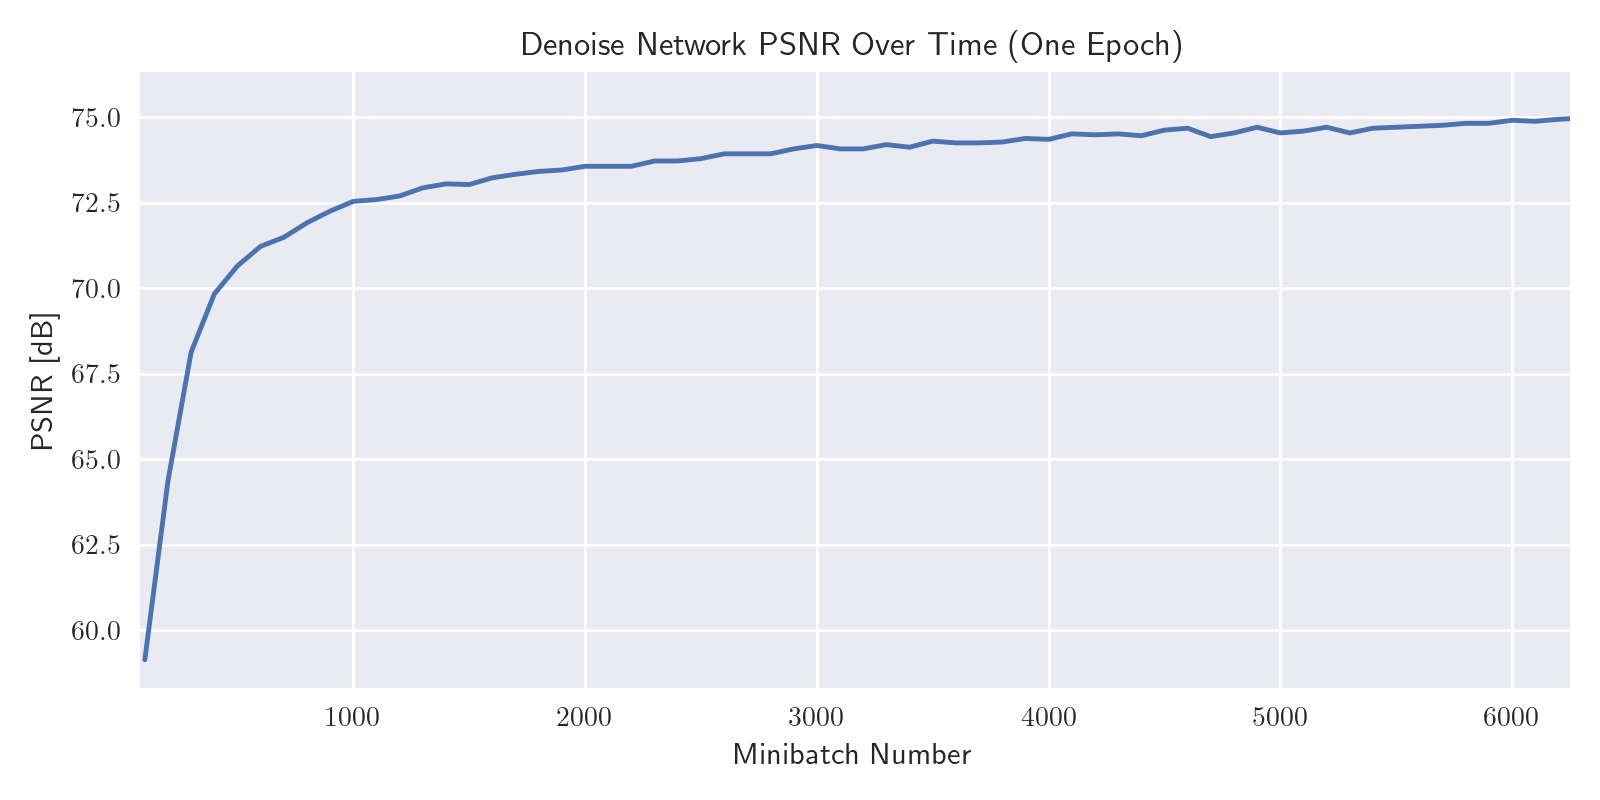
\includegraphics[width=0.8\textwidth]{figures/denoise-psnr}
    \caption{Denoising PSNR over time during training.}
    \label{fig:denoise-psnr}
  \end{figure}

  A example of the denoising network output image is shown in Figure \ref{eq:denoise-example}.
  Judging from the solid background, the denoising network appears to filter out Gaussian noise successfully as well as correct for the increased brightness to some degree.
  This agrees with the high PSNR the model achieved on the validation set was able to achieve.

  Note that the error is low in the uniform regions of the man's jacket and concentrated where the highly detailed regions are---the man's face and instrument.
  This example suggests the denoising network learned a lowpass filter to blur the input.

  \begin{figure}[H]
    \centering
    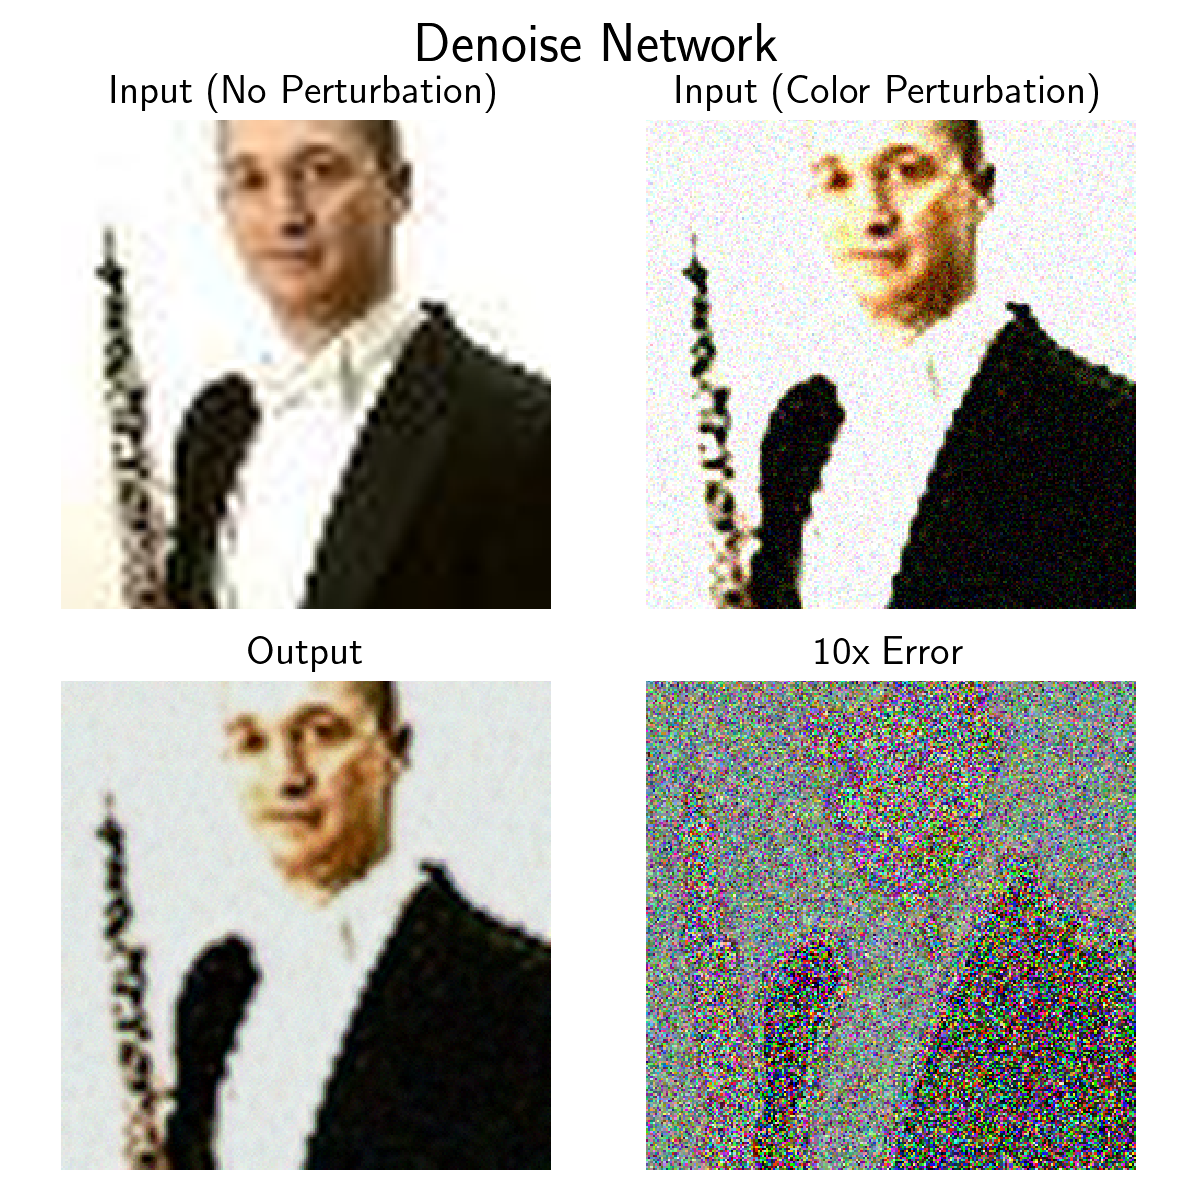
\includegraphics[width=0.6\textwidth]{figures/denoise.png}
    \caption{
      Example of denoise network output.
    }
    \label{eq:denoise-example}
  \end{figure}

  \section{Tools}

  We implemented our models in \href{https://pytorch.org/}{PyTorch}, a popular deep learning framework that offers standardized, performant implementations of learning primitives such as tensors, fully connected and convolutional layers, optimizers, and loss functions.
  Off-the-shelf support for GPUs made training high-capacity models computationally feasible.

  % We also used Google Colab for model training as they provide free compute-optimized resources such as GPUs (K80s, P100s, among others). Some training was also performed in Google Compute Engine and AWS EC2 instances, utilizing V100 GPUs. Also, PyTorch Tutorials from pytorch.org are launchable in Colab which was helpful for testing new ideas and getting a grasp on the API.

  PyTorch also has a vision submodule with common image transformations, which we used extensively in our data augmentation, and parameters for popular pretrained models.
  % From our experiments, models trained from scratch tended to underperform models pretrained on diverse datasets whose final fully connected layer we could fine-tune.
  % We hypothesize this performance gap exists because the early convolutional layers of the pretrained model have been trained on larger and more diverse datasets, so its layers are better at recognizing common low-level features of images like edges.

  We used Google Colab and virtual machines from Amazon Web Services and Google Cloud Platform for accelerating training with NVIDIA's Tesla V100 and P4 GPUs.

  \section{Lessons Learned}

  In summary, we have learned that data augmentation has a regularizing effect by effectively generating new training samples from the existing ones, which lowers overall model variance.
  Of course, the tradeoff is that the augmented samples may not accurately reflect either the original training set or the validation or test sets, as was the case with erasures, which injects noise into training and can hinder learning.

  We

  % Selecting a bad learning rate can cause a model to fail to make full use of its capacity.
  % Na\"{i}ve schemes like an exponentially decaying learning rate did not work particularly well because it's hard to tell \textit{a priori} what the base learning rate and the decay rate should be.
  % Adaptive schemes, such as the one-cycle learning rate policy, tended to work better because

  \section{Team Contributions}

  \begin{itemize}
  \item
    Jonathan Lee built, trained, and evaluated the denoising network.
    He wrote the training script and designed the perturbations.
    Estimated contribution: 40\%.
  \end{itemize}

  The code for this project is hosted on GitHub: \texttt{https://github.com/rchunter/CS182-ZouLeeGalHun}.

  The model parameters are located in this Google Drive folder:

  \texttt{https://drive.google.com/drive/u/1/folders/13K4ztT7Z2v7TYJgB1g0KPVCRp1u-K4tC}

  \bibliographystyle{unsrt}
  \bibliography{report}
\end{document}
